% Last updated in April 2018 by S. Hamid Rezatofighi
% Based on CVPR 07 and LNCS style, with modifications by DAF, AZ and elle 2008, AA 2010, ACCV 2010

\documentclass[runningheads]{llncs}
\usepackage{graphicx}
\usepackage{amsmath,amssymb} % define this before the line numbering.
\usepackage{ruler}
\usepackage{color}
\usepackage{multirow}
\usepackage{cite}
%===========================================================
\begin{document}
\pagestyle{headings}
\mainmatter

\def\ACCV18SubNumber{536}  % Insert your submission number here

%===========================================================
\title{ Recurrent Aggregation of Convolutional Neural Network} % Replace with your title
\titlerunning{ACCV-18 submission ID \ACCV18SubNumber}
\authorrunning{ACCV-18 submission ID \ACCV18SubNumber}

\author{Anonymous ACCV 2018 submission}
\institute{Paper ID \ACCV18SubNumber}

\maketitle

%===========================================================
\begin{abstract}
Standard convolutional neural networks assemble multiple convolutional layers to extract high-level features. Recent efforts keep designing deeper and wider architectures. Even with skip connections applied to combine different layers, the useful low-level features are not effectively utilized. Some deep layer aggregation methods have been proposed to aggregate features of all levels, using simple linear combination or complex non-linear transformation. In this paper, we treat convolutional features as a sequence, and propose our Recurrent Aggregation of Convolutional Neural Network (CNN-RA). Our aggregation method splits a standard CNN into blocks and maps their feature matrices to a sequence of vectors of the same length. LSTM is employed to connect to the sequence and better fuse features across blocks. Our proposed CNN-RA can be directly appended to any standard CNN without any modifications. Experiments show remarkable improvements of CNN-RA over the original architectures across datasets.
\end{abstract}

%===========================================================
\section{Introduction}

In recent years, Convolutional Neural Networks (CNNs) have shown remarkable advantage on computer vision tasks such as image classification\cite{imagenet}, object detection\cite{faster-r-cnn} and semantic segmentation\cite{refinenet}. The basic architecture of convolutional layer consists of two levels, feature extraction and feature mapping. In feature extraction level, the input of each convolutional neuron is connected to local receptive domain and the local characteristics are extracted. Feature mapping level employs multiple convolutional kernels to focus on different aspects of the characteristics. The results of different convolutional layers are customarily regarded as features containing spatial and channel-wise information. A series of convolutional layers are stacked together to expand the field of reception and to generate higher level features. The evolution of CNNs from LeNet\cite{lenet}, AlexNet\cite{alexnet} to ResNet\cite{resnet} and DenseNet\cite{densenet} increases both the performance and the size of the network, which yields deeper and wider network structures.

From the first application in ResNet\cite{resnet}, skip connections have been introduced into CNN structures, and proven effective on various vision tasks. Skip connections combine the output of previous layer and the current layer to deal with the gradient vanishing problem. DenseNet\cite{densenet} connects densely in a block to make better use of previous features. To further utilize features from different layers, Yu\cite{dla} extends the current skip connection approach and proposes deep layer aggregation (DLA) architectures. These architectures simply combine features of different level by concatenation or addition, without considering the interior relationship between low-level and high-level feature representations. 

Recurrent Neural Networks (RNNs)\cite{rnn} have been proposed to deal with sequential data like text and speech. Different from feedforward neural networks, RNNs build connections between neurons which are in the same layer. RNNs can be unfolded as a directed graph along the time steps, with all the layers sharing the same weights. This makes RNNs applicable to sequential tasks such as text classification. Long Short Term Memory (LSTM)\cite{lstm} is a special RNN, which makes use of three gates to select valuable information from all the memories. LSTM has proven to be more efficient than normal RNNs in most tasks on sequences.

In this work, we propose a brand new approach to convolutional layer aggregation, by introducing a new architecture which is named as '\emph{Convolutional Neural Network-Recurrent Aggregation}' (CNN-RA).  Our goal is to use LSTM to aggregate outputs of multiple layers and retrieve more expressive features. To achieve this, we build CNN-RA by creating parallel connection between a CNN and a LSTM. Features from lower convolutional layers to higher layers naturally form a sequence with a various granularity of information. This kind of sequence contains both the features themselves and the transformation relationship between different levels of features, which directly leads us to RNNs. We create information between outputs of convolutional layers and the inputs of LSTM, and employ the outputs of LSTM as the final feature for tasks such as image classification.

The receptive fields and feature maps sizes of different convolutional layers vary from each other, especially for consecutive layers with a pooling layer in-between. We propose an algorithm to transform different shape of feature matrices to vectors with the same dimension. Then transformed vectors are stacked together as inputs of LSTM. The number of chosen features is the step length of the LSTM.

The development of new network architectures is always a time consuming task with abundant hyper parameters to determine. Previous work on layer aggregation such as DLA\cite{dla} brings with huge change on the original network architecture, which can even be much more complicated. However, our proposed CNN-RA won't do any modification on the original network, by only connecting it with a parallel LSTM. This property enables CNN-RA to be easily applicable to multiple convolutional network structures. 

Our evaluation experiments extend famous network structures VGGNet\cite{vgg} and ResNet\cite{resnet} for image classification task on benchmark datasets. The testing results show improvements across different network structures and datasets over other state-of-the-art aggregation methods. The connected LSTM brings with higher performance without increasing much in parameter numbers. The experiment processes show that the relationship between two convolutional blocks with a down sampling layer inside has the most important contribution to the model.

%Do not use any additional Latex macros.

%------------------------------------------------------------------------- 

\section{Related Work}
Convolutional neural networks (CNNs) have proven their great advantage on computer vision tasks. The successful application of LeNet\cite{lenet} and AlexNet\cite{alexnet} on ImageNet\cite{imagenet} classification tasks first demonstrated the effectiveness of convolutional architecture for visual recognition. Inspired by the combination of convolutional, pooling and full-connected layers, VGGNet\cite{vgg} proposed to assemble several layers with small convolutional kernels to replace a large kernel. It achieved huge improvement over AlexNet on almost every visual problem. ResNet\cite{resnet} employed residual blocks to avoid vanishing gradient problem and enabled very deep network to work well. Skip connection was also first proposed in ResNet and helped improve performance over various visual problems. DenseNet\cite{densenet} was an advanced edition of skip connection, because it connected each two layers within a block to maximize the data flow. DenseNet made better use of information within a block and show excellent accuracy over image classification tasks. CliqueNet\cite{cliquenet} increased the complexity by proposing clique blocks. It applied bi-directional connection between each two layers in a block and built a bi-directional fully connected graph. CliqueNet made block layers recurrent and was denser than DenseNet.

Recurrent neural networks (RNNs) have been designed to deal with sequential data, which build connections between units in each layer. RNN was first proposed by \cite{rnn} to learn long term dependencies. The architecture was designed to capture the contextual information and has been successfully applied in text recognition\cite{text_rnn}, automatic speech recognition\cite{speech_rnn} and video processing\cite{video_rnn}. Long-short Term Memory (LSTM)\cite{lstm} employed forget gate to consider both short-term and long-term memory.  It was capable of remembering the long-term information and extracting effective information from a long sequence. Bi-directional LSTM (BLSTM)\cite{blstm} focused on the imperfection of LSTM which only took previous information into consideration. BLSTM employed two LSTM structure with opposite direction and fused information of the whole sequence.

Layer aggregation fuses information of different layers to better utilize the features. FCN\cite{FCN}, FPN\cite{FPN} and U-Net\cite{U-Net} employed simple skip connection to combine cross-layer information, which directly connected shallow layers to the end. Deep Layer Aggregation\cite{dla} proposed iterative deep aggregation (IDA) and hierarchical deep aggregation (HDA). IDA iteratively merged lower layers and deeper layers, to aggregate shallower features more sufficiently. This  helped refine shallow features. HDA merged convolutional blocks in a tree, and combined different layers in parallel as well as in series. However, DLA made the network structures very complicated and did not aggregate features of different levels innovatively. The main idea of DLA is still skip connections ever different layers and stages.

\section{Methodology}
Convolutional layer aggregation is a combination of features from different layers. The output matrices of convolutional layers are regarded as expressive features for vision tasks. In general, shallow layers contain low-level features and deep layers contain high-level features. Existing work simply uses high-level features or a combination of all layers. In this work, we take into account both feature combination and the sequential transformation relationship between all levels. Output features of convolutional layers form a sequence and RNNs are designed to deal with sequential data. LSTM is employed to do the layer aggregation on CNN in this paper. The output shape of different layers varies, therefore we use mapping nodes to map selected features to the same dimension first, and then aggregate them to be the input of LSTM. The structure diagram of CNN-RA is shown in Fig.~\ref{fig:CNN-RA}.

Recent network design tends to assemble several blocks together and simplifies the network representation. Several layers are grouped into a single block which is capable of realizing some feature extraction and transformation function. Our proposed aggregation method employs the output of blocks instead of all layers to focus on useful but not redundant information. 

\begin{figure}  
	\centering
	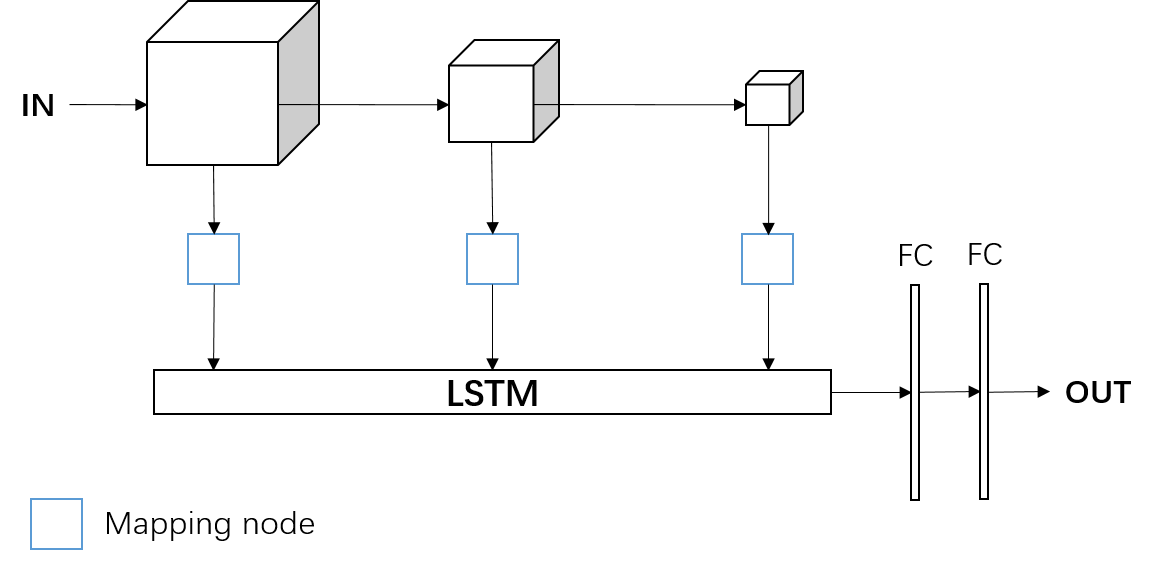
\includegraphics[width=12cm]{Figures/CNN-RA.png}
	\caption{Structure of CNN-RA}
	\label{fig:CNN-RA}
\end{figure}

\subsection{Convolutional Feature Mapping}

Convolutional feature mapping helps transform feature matrices of different blocks into vectors with the same dimension. The feature resolution and number of channels vary among blocks because of convolution and down-sampling operations. Then the blocks are grouped into stages according to their output shape. Blocks within the same stage share common mapping operation which is different from other stages. In general, deeper layer holds smaller feature resolution and more channels. We propose to take the feature tensor of the last block as the standard $S \in \mathbb{R}^{H\times W \times C}$ and transform other matrices towards its dimension. 

The standard $S$ contains high-level features and each unit of $S$ holds a large receptive field size due to previous convolution and down-sampling operations. For such output features we tend to exploit their channel dependencies instead of total information. Therefore, we do global average pooling on $S$ to squeeze the spatial information into a channel-wise vector. Then a channel descriptor $D\in \mathbb{R}^C$ is generated with the $c_{th}$ element $D_c$ calculated by:
\begin{equation}
D_c = F_{gp}(S_c) = \frac{1}{H\times W}\sum_{i=1}^H\sum_{j=1}^W S_c(i,j).
\end{equation}

Shallow blocks, where each unit can cover a limited region of receptive field, contain local information and this information helps extract fine features. Our proposed layer aggregation pays attention to both low-level and high-level features,  and thus global average pooling operation is not suitable for these shallow blocks. We embed a convolutional layer with kernel size $k\times k$ and stride $l=k$ to combine local information, and then use average pooling layer with kernel size equal to the feature map shape of $S$.  An output matrix $U\in \mathbb{R}^{h\times w\times c}$ is generated with $h\times w\times c=C$.  We then expand the matrix $U$ to a vector with the same length as $D$.

The receptive fields of  blocks in middle stages are large enough to cover the input image, and the numbers of channels are normally less than $C$. For these kinds of blocks, we first embed a convolutional layer with channel number $C$ to extend the channel number, and then take global average pooling on the output. A vector with length $C$ is then generated.

The generated vectors share the same length and can be arranged into a matrix. Given a network structure with $N$ blocks, we can generate a feature matrix $V\in \mathbb{R}^{N\times C}$.

\subsection{Recurrent Aggregation using LSTM}
After convolutional feature mapping we get a matrix $V\in \mathbb{R}^{N\times C}$. The matrix is constructed by assembling a sequence of $N$ feature vectors $v \in \mathbb{R}^{1\times C}$ and we denote $V=[v_1, v_2, \cdots, v_N]$. As shown in Fig.~\ref{fig:CNN-RA}, the sequential vectors are arranged according to the generated order in the CNN structure, and $[v_1$ to $v_N]$ denote features from low-level  to high-level. 
\begin{figure}  
	\centering
	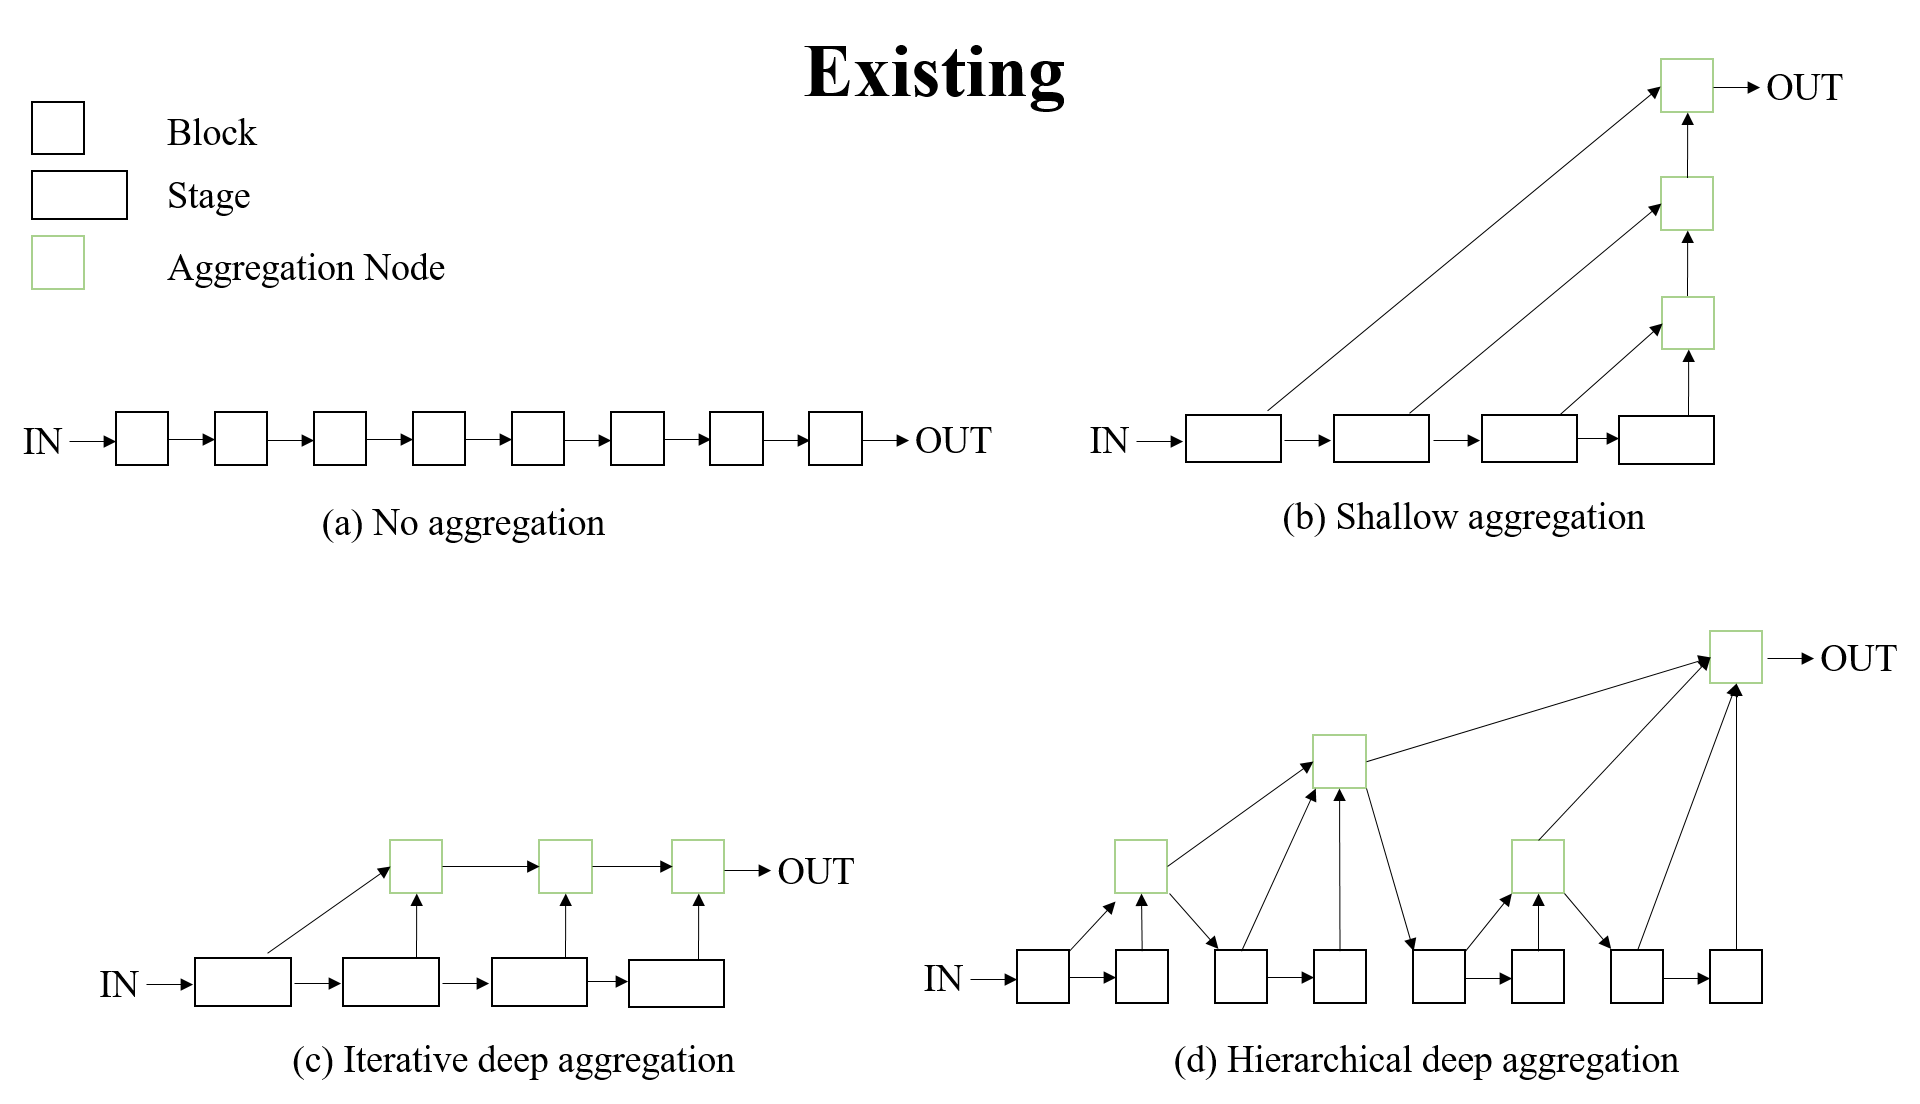
\includegraphics[width=13cm]{Figures/existed_aggr.png}
	\caption{Different existing approaches to aggregation. (a)default classification and regression networks without aggregation. (b)shallow linear combination of all layers by skip connection. (c)iterative deep aggregation to better aggregate shallow layers. (d)hierarchical deep aggregation to better preserve previous features.}
	\label{fig:exited_aggr}
\end{figure}
Existing work on convolutional layer aggregation focuses on the linear and non-linear combination of different layers. Fig.~\ref{fig:exited_aggr}(b) shows the shallowest aggregation, which simply makes linear combination on all blocks. Yu\cite{dla} proposed iterative deep aggregation (IDA) and hierarchical deep aggregation (HDA) as shown in Fig.~\ref{fig:exited_aggr}(c) and Fig.~\ref{fig:exited_aggr}(d).  IDA iteratively merges lower layers with deeper layers to refine shallow features. HDA employs deep and branching structure to better preserve features.

Recurrent aggregation of CNN (CNN-RA) merges blocks as a sequence to both contain the spatial and channel-wise information and explore the transformation relationship according to the order. The mapped feature vectors share the same length and form a regular sequence. One typical sequential data is text, and RNN has shown their tremendous advantage on processing text data. The successful application of RNNs mainly relies on their memory on contextual information. The memory mechanism helps combine all the input information together and is capable of detecting the correlation among all steps. LSTM employs input gate, forget gate and output gate to realize the long short-term memory, which naturally introduces attention mechanism to focus on useful information. LSTM takes input of $n$ steps, with all the input vector sharing the same dimension and the mapped feature matrix $V\in \mathbb{R}^{N\times C}$ satisfies the requirements. The output vector of LSTM $U$ can be calculated by:
\begin{equation}
U = F_{LSTM}(V)
\end{equation}
where $F_{LSTM}$ denote a standard LSTM structure with forget gates. The inputs of LSTM connect to the convolutional blocks through mapping nodes, and the gradient can be directly back propagated to all the blocks. These connections contribute to avoiding vanishing gradient problem and help convolutional blocks to extract more expressive sequential features.

The output vector $U$ of LSTM contains squeezed and abstract information through the convolutional network. To utilize this abstract feature, we embed a simple non-linear combination before the output layer as:
\begin{equation}
u = \sigma(WU)
\end{equation}
where $\sigma$ denote the ReLU\cite{ReLU} function. 

\subsection{Examples: VGG-RA and ResNet-RA}
The flexibility of recurrent aggregation using LSTM means that it can be directly appended to standard convolutional neural networks, without any modification on the original structure. Given a normal CNN, all we need to do is selecting output features to be employed, mapping them to vectors with the same length and arrange them into a matrix as the input of LSTM. In this paper, we apply CNN-RA to modern architectures VGGNet and ResNet to show the efficiency.

For non-blocked networks such as VGGNet, feature selection needs to be done before layer aggregation. In general, modern CNN architectures repeat serval convolution followed by a down-sampling operation to extract features. We classify the convolutional layers sharing the same feature resolution into the same stage, and split each stage into 1 or more blocks manually. Then the network is grouped into blocks with each blocks containing more than one convolutional layers. We construct VGG-RA network by simply choose the first three stages of VGGNet and aggregate it with a LSTM network. The VGG-RA network structure is shown in Fig.~\ref{fig:VGG-RA}.
\begin{figure}  
	\centering
	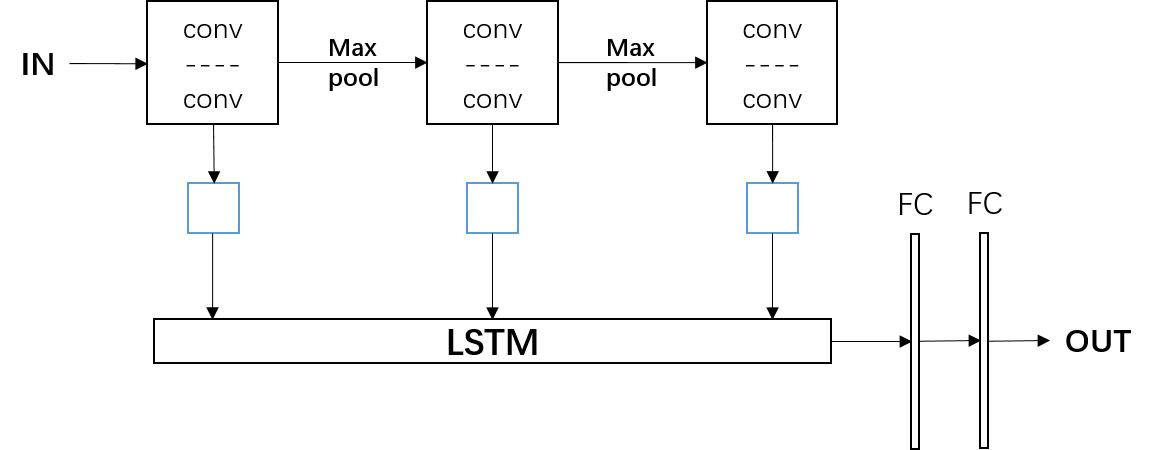
\includegraphics[width=11cm]{Figures/VGG-RA.png}
	\caption{Structure of VGG-RA}
	\label{fig:VGG-RA}
\end{figure}

Blocked networks like ResNet are easy to apply CNN-RA, with each block outputing a feature matrix. For complex blocks such as a residual block with 20 or more convolutional layers, we can also split them into more sub-blocks. We employ ResNet with 3 residual blocks to build ResNet-RA, and the structure diagram is shown in Fig.~\ref{fig:ResNet-RA}.
\begin{figure}  
	\centering
	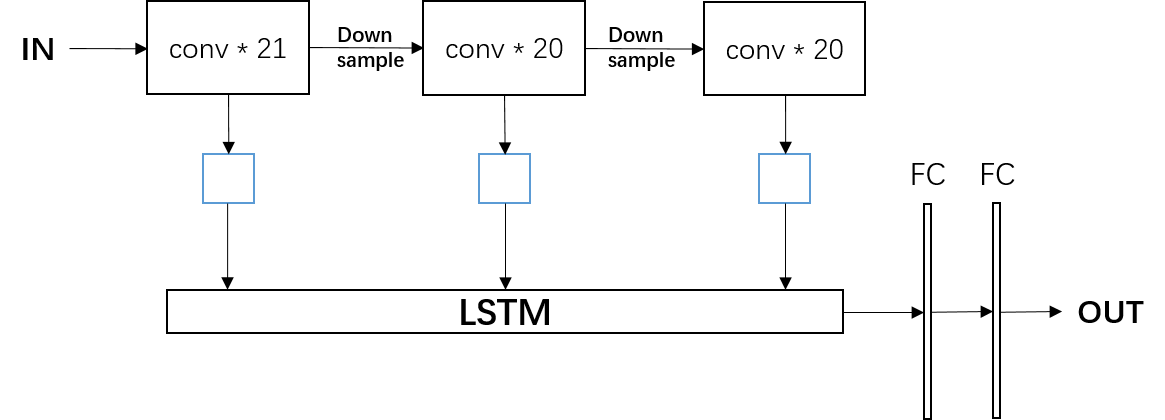
\includegraphics[width=11cm]{Figures/ResNet-RA.png}
	\caption{Structure of ResNet-RA}
	\label{fig:ResNet-RA}
\end{figure}

\section{Training Details}
\subsection{Feature selection}
Given a standard CNN structure, we just select some of the convolutional layers to be aggregated. A large number of outputs bring with complexity and much redundant information, which brings down the appearance and convergence rate of LSTM. The selected blocks have to satisfy three rules we proposed: (a)each block contains at least 2 convolutional layers, (b)each stage contains at most 2 blocks, (c)the selected layer in each stage should be located before the corresponding down-sampling layer. According to these three rules, we split VGGNet and ResNet into 3 blocks, which is shown in Table~\ref{table:struc}.
\subsection{Feature Mapping}

Feature mapping nodes transform the feature matrix of CNN layers to the input vectors of LSTM. The feature resolution and channel number vary from shallow layers to deep layers, however, LSTM requires inputs of a common dimension. We first take global average pooling on the last block output and generate a standard vector. In general, previous blocks hold larger feature map and fewer channels. We propose to treat different blocks according to their feature resolutions, and group them into three levels, shallow level, middle level and last level. The last level only contains the final block. The middle level contains blocks whose feature resolutions is $2\times$ or $1\times$ larger than that of the final blocks. The shallow blocks contains the rest blocks. 

The last block outputs a standard vector $v_e$ with the same dimension as the last channel number $C$ by global average pooling. For middle level blocks, we employ a single convolutional layer to transform the feature resolution and channel number into the same as the final block and then take the global average pooling operation. Blocks in shallow levels are handled specially, because their feature resolutions are at least $4\times$ larger than the final block and the receptive fields may not cover the input size. These blocks contain more details information which we hope to utilize. Thus we first combine the spatial information by a convolutional layer with stride 2, and take average pooling with the kernel size equal to the shape of the final block. A feature matrix $u \in \mathbb{R}^{h\times w \times c}$ is then generated with $h\times w \times c = C$ and is expanded to $v_s$. All feature vectors are arranged into a matrix $V$ as the input of LSTM.

\subsection{Implementation Details}

We verify the effectiveness of CNN-RA on three famous classification benchmark Cifar10\cite{cifar}, SVHN\cite{SVHN} and Cifar100\cite{cifar}. All these three datasets contain images with size $32\times 32\times 3$. We do data augmentation on Cifar10 and Cifar100 by first resizing the images to $40\times 40\times 3$ and then randomly cropped them to $32\times 32\times 3$. We also flip the images at random.

Considering the small resolution of images, we do some manipulation on the original network structure. Standard VGGNet consists of five down-sampling layers and cannot be directly applied to small images. We select the first three stages with each containing two convolutional layers and a pooling layer, which we denote as VGG-1 in this paper. The selected network contains totally 6 convolutional layers and we group them into 3 blocks with each containing 2 layers. VGG-1 is shallow and each stage contains only two layers. We then double each block to 4 layers and generate a new network denoted as VGG-2. VGG-2 contains 12 layers and is also grouped into 3 blocks according to their feature resolutions. ResNet is block-wise and we assemble three blocks with each containing 20 convolutional layers. To eliminate the influence of complexity by applying LSTM, we embed a fully-connected layers before output layer in the re-implementation.

We apply CNN-RA to the three networks by appending a normal LSTM structure. The aggregated network is then correspondingly denoted as VGG-1-RA, VGG-2-RA and ResNet-RA. The structure parameters are listed in Table~\ref{table:struc}. We employ Batch-Normalization in each model to accelerate the convergence, and learning rate decay to optimize the convergence results.

\setlength{\tabcolsep}{4pt}
\linespread{1.2}
\begin{table}
\begin{center}
\caption{
Network parameters of re-implementation and aggregation. GAP denotes global average pooling.
}
\label{table:struc}
\begin{tabular}{l|l|l|l|l}
\hline\noalign{\smallskip}
Network& Block1 & Block2 & Block3 & Classifier\\
\noalign{\smallskip}
\hline
\noalign{\smallskip}
VGG-1 & conv,128 $\times$ 2 & conv,256 $\times$ 2 & conv,512 $\times$ 2 & 1024d-fc$\times$2, softmax \\
\hline
VGG-2 & conv,128 $\times$ 2 & conv,256 $\times$ 2 & conv,512 $\times$ 2 & 1024d-fc$\times$2, softmax \\
\hline
ResNet & conv,64 $\times$ 21 & conv,128 $\times$ 20 & conv,256 $\times$ 20 & GAP, 256d-fc, softmax \\
\hline
\multirow{2}{*}{VGG-1-RA} & conv,128 $\times$ 2 & conv,256 $\times$ 2 & conv,512 $\times$ 2 & \multirow{2}{3cm}{256d-fc, softmax} \\
\cline{2-4}
					 & \multicolumn{3}{c|}{LSTM 256} \\
\hline
\multirow{2}{*}{VGG-2-RA} & conv,128 $\times$ 2 & conv,256 $\times$ 2 & conv,512 $\times$ 2 & \multirow{2}{3cm}{256d-fc, softmax} \\
\cline{2-4}
					 & \multicolumn{3}{c|}{LSTM 256} \\
\hline
\multirow{2}{*}{ResNet-RA} & conv,64 $\times$ 21 & conv,128 $\times$ 20 & conv,256 $\times$ 20 &\multirow{2}{3cm}{256d-fc, softmax} \\
\cline{2-4}
					& \multicolumn{3}{c|}{LSTM 256}\\
\hline
\end{tabular}
\end{center}
\end{table}
\setlength{\tabcolsep}{1.4pt}

\section{Results}

\subsection{Classification with CNN-RA}

We evaluate our recurrent aggregation methods on three image classification benchmark datasets Cifar10, SVHN and Cifar100 using three standard networks. We first re-implement VGG-1, VGG-2 and ResNet shown in Table~\ref{table:struc}, and train them on the three datasets. The networks are trained by SGD with momentum 0.9. We set weight decay as $10^{-4}$ and batch size as 64. For all the three datasets, we train 100 epochs. For Cifar10 and SVHN, the learning rates starts at 0.01, and is reduced by 10 at $50_{th}$ and $75_{th}$ epoch. For Cifar100, the learning rates starts at 0.005 and is reduced at $80_{th}$ epoch. The data augmentation is operated on Cifar10 and Cifar100 with random-cropping and flipping. Then we evaluate the trained model on the three test sets and take the results as the baselines and are shown in Table~\ref{table:test}.

After the training and evaluation of the re-implemented network, we build VGG-1-RA, VGG-2-RA and ResNet-RA by joining LSTM and the original network with mapping nodes. To be fair, we train the aggregated network with the same procedure and hyper-parameters. We evaluate our aggregated network on the three test sets, and the results are shown in Table~\ref{table:test}.
\setlength{\tabcolsep}{4pt}
\begin{table}
\begin{center}
\caption{Validation accuracies on three datasets. The number in parenthesis represents the improvements of network with CNN-RA over the original network.}
\label{table:test}
\begin{tabular}{l|lll}
\hline\noalign{\smallskip}
Network& Cifar10 & SVHN & Cifar100\\
\noalign{\smallskip}
\hline
\noalign{\smallskip}
VGG-1 & 93.73 & 97.97 & 73.01\\
VGG-1-RA & 94.49(0.76)$\quad$ & 98.11(0.14)$\quad$ & 74.81(1.80)\\
VGG-2 & 94.91 & 98.14 & 75.66\\
VGG-2-RA & 95.30(0.39) & 98.32(0.18) & 77.48(1.82)\\
ResNet & 93.74 & 98.00 & 75.87\\
ResNet-RA & 94.78(\textbf{1.04}) & 98.19(\textbf{0.19}) & 77.85(\textbf{1.98})\\
\hline
\end{tabular}
\end{center}
\end{table}
\setlength{\tabcolsep}{1.4pt}

In Table~\ref{table:test}, the digits represent the improvement on testing accuracy of networks with CNN-RA over the original ones. For all three networks over the three benchmark datasets, our proposed recurrent aggregation method makes improvements. On Cifar10, ResNet-RA achieves over 1\% on testing accuracy. On Cifar100, all the three networks with CNN-RA achieves more than 1\% improvements, and ResNet-RA even increase remarkably 1.98\%.

These comparison experiments show the effectiveness of CNN-RA. Considering the complexity and difficulty of the datasets themselves, Cifar100 contains 100 classes while Cifar10 and SVHN contains 10. The otherness of intra-class images in Cifar10 is much larger than SVHN. Thus we rank them as Cifar100, Cifar10 and SVHN according to their complexity. The testing results show that, all these three networks show better performance on simple datasets over the complex one, and networks with CNN-RA show the same phenomenon. Paying attention to the improvements on the three datasets and we notice that, the increment of accuracy of three networks is larger when the task is more complex. The improvement on SVHN is less than 0.2\%, and that of Cifar10 achieves 1.04\%, while the accuracy increases up to 1.98\% over Cifar100. The difference of testing results is caused by two reasons. The first is that these networks are capable to deal with simple tasks well, and the upside potential is relatively smaller than the complex tasks. The second reason is concluded as the effectiveness of information aggregation. For simple tasks such as SVHN classification, high-level features are enough to distinguish different classes. However, for complex problems like Cifar100, the intra-class information is complicated with backgrounds and a variety samples of the same class. Then we need to utilize the features from low-level to high-level and their combination patterns. The results indicate that the recurrent aggregation method works better on more complex tasks. Another remarkable fact is that, the CNN-RA shows better results on ResNet which has totally 61 layers. In ResNet, each block contains 20 convolutional layers, which brings significant difference between two blocks. CNN-RA seems to work better on capturing feature transformation relationship of deeper blocks.

\begin{figure}   
	\centering
	\includegraphics[width=8cm]{Figures/cifar10.png}
	\caption{Testing Accuracy on Cifar10}
	\label{fig:Cifar10}
\end{figure}
\begin{figure}  
	\centering
	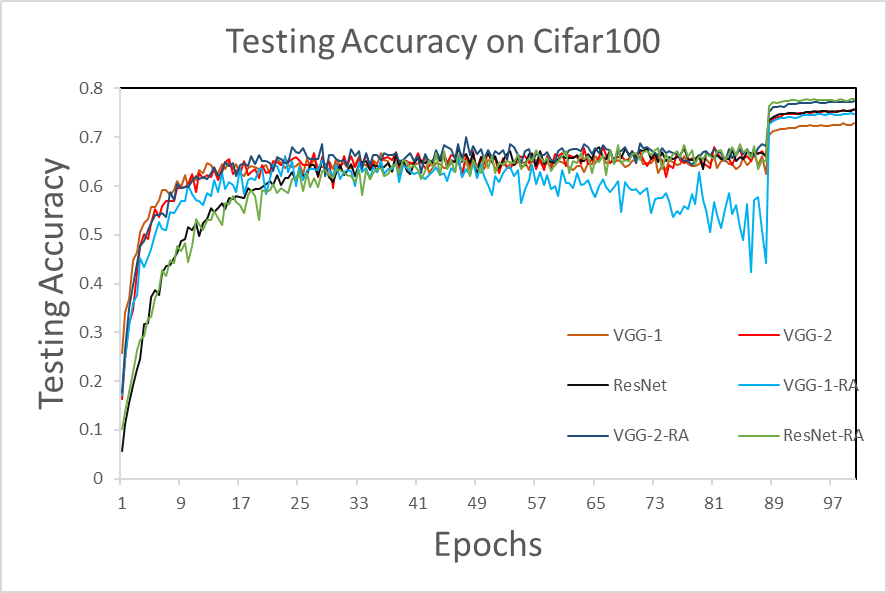
\includegraphics[width=8cm]{Figures/cifar100.png}
	\caption{Testing Accuracy on Cifar100}
	\label{fig:Cifar100}
\end{figure}

Our model takes different learning decay between Cifar10, SVHN and Cifar100. In Fig.~\ref{fig:Cifar10} and Fig.~\ref{fig:Cifar100} we show the training procedure on Cifar10 and Cifar100. It can be seen that, on Cifar10, recurrent aggregation method helps the network converge faster and show better final results. On Cifar100, all the three networks converge slower at the beginning with CNN-RA, however, they achieve higher performance after learning rate decay. ResNet-RA increases the most at the learning rate decay point. These learning curves show the different effect of CNN-RA on various tasks. For simple tasks, networks with aggregation converge faster and achieve better results in the end. For complex tasks, recurrent aggregation brings with lower convergence but higher accuracy eventually. The appended LSTM helps extract more expressive features, and it takes longer to better fit the complex dataset.


\subsection{More Explorations}
To better understand the effectiveness of our proposed CNN-RA, we explore some other methods to employ the outputs of LSTM.
\begin{figure}   
	\centering
	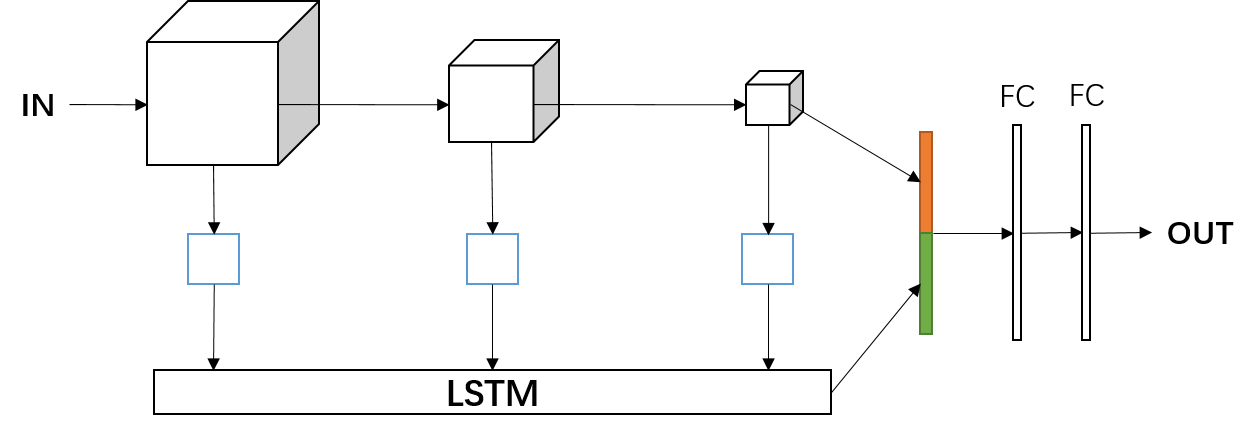
\includegraphics[width=11cm]{Figures/RA-B.png}
	\caption{Structure of CNN-RA-B}
	\label{fig:CNN-RA-B}
\end{figure}
\begin{figure}  
	\centering
	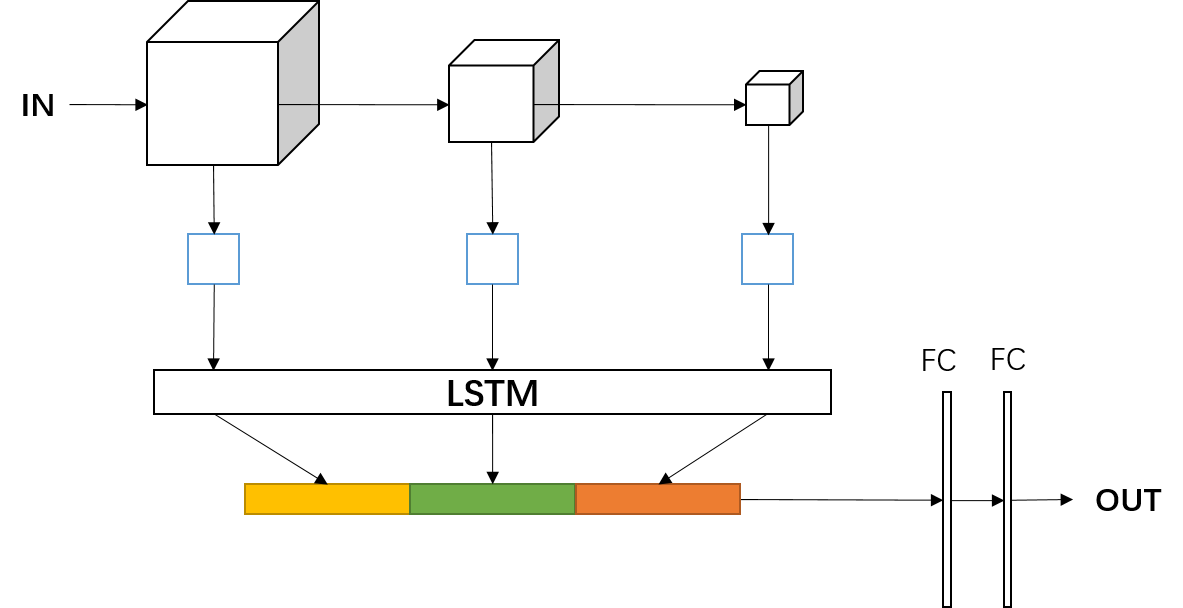
\includegraphics[width=11cm]{Figures/RA-C.png}
	\caption{Structure of CNN-RA-C}
	\label{fig:CNN-RA-C}
\end{figure}

Given a network with $N$ blocks, we employ a LSTM with $N$ steps to aggregrate the features. In Fig.~\ref{fig:CNN-RA}, only the final state is considered and directly used to do the classification. Fig.~\ref{fig:CNN-RA-B} show a combination of aggregated feature and the original high-level feature. We concatenate the output of LSTM and the feature vector of the last block as a new vector, and apply it to the classifier. We denote this structure as CNN-RA-B. In Fig.~\ref{fig:CNN-RA-C}, we concatenate the corresponding $N$ output vectors together as the final feature, and employ it for classification. We denote the structure as CNN-RA-C.


To evaluate the performance of these two transformative network structures, we employ ResNet as the baseline and test on all three dataset. The evaluation results are shown in Table~\ref{table:RA-B-C}. CNN-RA improves the performance of ResNet on all three datasets. The combination of aggregated features and the original high-level features at least maintains the accuracy of ResNet, and shows obvious advantage over Cifar10. However, the results of ResNet-RA-B are worse than ResNet-RA over all three datasets. This is probably because the propagation through the original architecture is more straightforward than the aggregated structure and the aggregated features are suppressed during the training process and only play a weak role on the task. ResNet-RA-C concatenates output features of all steps in LSTM to further combine low-level to high-level information. The output of LSTM naturally relates to the information containing previous steps. The structure shows remarkable improvement on SVHN, and is even better than ResNet-RA. However, on Cifar10 and Cifar100, ResNet-RA-C just shows small advantage, and is even worse than ResNet-RA-B. This might because in ResNet-RA-C, the shallow features are even directly employed to do the classification, and they bring much redundant information and has bad influence on the network performance.
\setlength{\tabcolsep}{4pt}
\begin{table}
\begin{center}
\caption{Validation accuracies of ResNet, ResNet-RA, ResNet-RA-B and ResNet-RA-C over three datasets.}
\label{table:RA-B-C}
\begin{tabular}{l|lll}
\hline\noalign{\smallskip}
Network& Cifar10 & SVHN & Cifar100\\
\hline
ResNet &93.74  &98.00  &75.87  \\
ResNet-RA  &94.78  &98.19  &77.85  \\
ResNet-RA-B  &94.42  &98.01  &75.91  \\
ResNet-RA-C  &93.85  &98.31  &75.89  \\
\noalign{\smallskip}
\hline
\noalign{\smallskip}

\end{tabular}
\end{center}
\end{table}
\setlength{\tabcolsep}{1.4pt}

These two explorations show some different methods of combining our recurrent aggregated features with other information. In these experiments, all structures achieve large or small improvements across networks and datasets. On the whole, ResNet-RA shows better performance than ResNet-RA-B and ResNet-RA-C, which definitely proves the effectiveness of our recurrently aggregated features.

\section{Conclusion}
In this paper, we propose a brand new method of convolutional layer aggregation method which is denoted as CNN-RA. Recurrent layer aggregation first splits a CNN into convolutional blocks and arranges their output features into a matrix. A LSTM is then employed to combine the low-level to high-level features and extract the sequential relationship between them. CNN-RA can be simply applied to any standard CNN without any modification on the original architectures. We evaluate our aggregation methods over Cifar10, SVHN and Cifar100 using VGG-1, VGG-2 and ResNet. The results show remarkable improvements with CNN-RA. Our proposed recurrent aggregation method is the first to put forward treating the convolutional layer features as a sequence and combining CNN and RNN parallelly together. The evaluation experiments verify the effectiveness of CNN-RA and show its great potential on utilizing the features in CNNs.
\newpage
%===========================================================
\bibliographystyle{splncs}
\bibliography{egbib}

%this would normally be the end of your paper, but you may also have an appendix
%within the given limit of number of pages
\end{document}
